\section{Results}
\label{sec:results}

\para{Pooled no-hint accuracy.} \Tabref{tab:no_hint} reports pooled results across all three datasets without misleading hints. Mild skeptical prompting produces the best pooled accuracy for \gptfourone at 69.2\%, up from 64.2\% under neutral prompting. The paired bootstrap 95\% confidence interval for this gain is [+0.8, +10.0] percentage points. Neither stronger judgment condition exceeds this result. For \gptfouronemini, pooled differences are smaller and less stable: mild skepticism and the strong judgment question both reach 64.2\%, only 1.7 points above neutral, while the strong judgment statement falls slightly below neutral.

\begin{table}[t]
    \centering
    \caption{Pooled no-hint results across \gsm, \csqa, and \truthfulqa. Higher accuracy is better. Best accuracy per model is shown in \textbf{bold}.}
    \label{tab:no_hint}
    \resizebox{\textwidth}{!}{%
    \begin{tabular}{@{}llccc@{}}
        \toprule
        Model & Condition & Accuracy & Mean rationale words & Mean confidence \\
        \midrule
        \gptfourone & Neutral & 0.642 & 31.84 & 96.91 \\
        \gptfourone & Mild skeptical question & \textbf{0.692} & 33.37 & 96.93 \\
        \gptfourone & Strong judgment question & 0.667 & \textbf{33.71} & 96.95 \\
        \gptfourone & Strong judgment statement & 0.658 & 32.34 & \textbf{97.12} \\
        \midrule
        \gptfouronemini & Neutral & 0.625 & 22.59 & \textbf{94.17} \\
        \gptfouronemini & Mild skeptical question & \textbf{0.642} & \textbf{25.43} & 92.58 \\
        \gptfouronemini & Strong judgment question & \textbf{0.642} & 25.21 & 92.92 \\
        \gptfouronemini & Strong judgment statement & 0.617 & 23.65 & 93.17 \\
        \bottomrule
    \end{tabular}%
    }
\end{table}


\para{Misleading-hint robustness.} \Tabref{tab:with_hint} summarizes the misleading-hint setting. Here the no-hint gain disappears. For \gptfourone, pooled accuracy drops from 81.2\% under neutral to 78.8\% under mild skepticism and 76.2\% under the strong judgment question. For \gptfouronemini, mild skepticism and the strong statement match neutral pooled accuracy at 73.8\%, while the strong judgment question is lower at 71.3\%. Wrong-hint agreement remains low across all conditions, ranging from 5.0\% to 6.2\% for \gptfourone and from 7.5\% to 10.0\% for \gptfouronemini. This pattern argues against a simple story in which harsher prompts directly make the models agree with the injected wrong answer more often.

\begin{table}[t]
    \centering
    \caption{Pooled results with misleading wrong hints on \csqa and \truthfulqa. Higher accuracy is better and lower wrong-hint agreement is better. Best accuracy per model is shown in \textbf{bold}.}
    \label{tab:with_hint}
    \resizebox{\textwidth}{!}{%
    \begin{tabular}{@{}llccc@{}}
        \toprule
        Model & Condition & Accuracy & Wrong-hint agreement & Mean rationale words \\
        \midrule
        \gptfourone & Neutral & \textbf{0.812} & 0.062 & 34.09 \\
        \gptfourone & Mild skeptical question & 0.788 & \textbf{0.050} & 35.69 \\
        \gptfourone & Strong judgment question & 0.762 & \textbf{0.050} & \textbf{35.79} \\
        \gptfourone & Strong judgment statement & 0.800 & 0.062 & 33.86 \\
        \midrule
        \gptfouronemini & Neutral & \textbf{0.738} & 0.100 & 23.91 \\
        \gptfouronemini & Mild skeptical question & \textbf{0.738} & \textbf{0.075} & 23.96 \\
        \gptfouronemini & Strong judgment question & 0.713 & 0.088 & \textbf{26.79} \\
        \gptfouronemini & Strong judgment statement & \textbf{0.738} & \textbf{0.075} & 24.28 \\
        \bottomrule
    \end{tabular}%
    }
\end{table}


\begin{figure}[t]
    \centering
    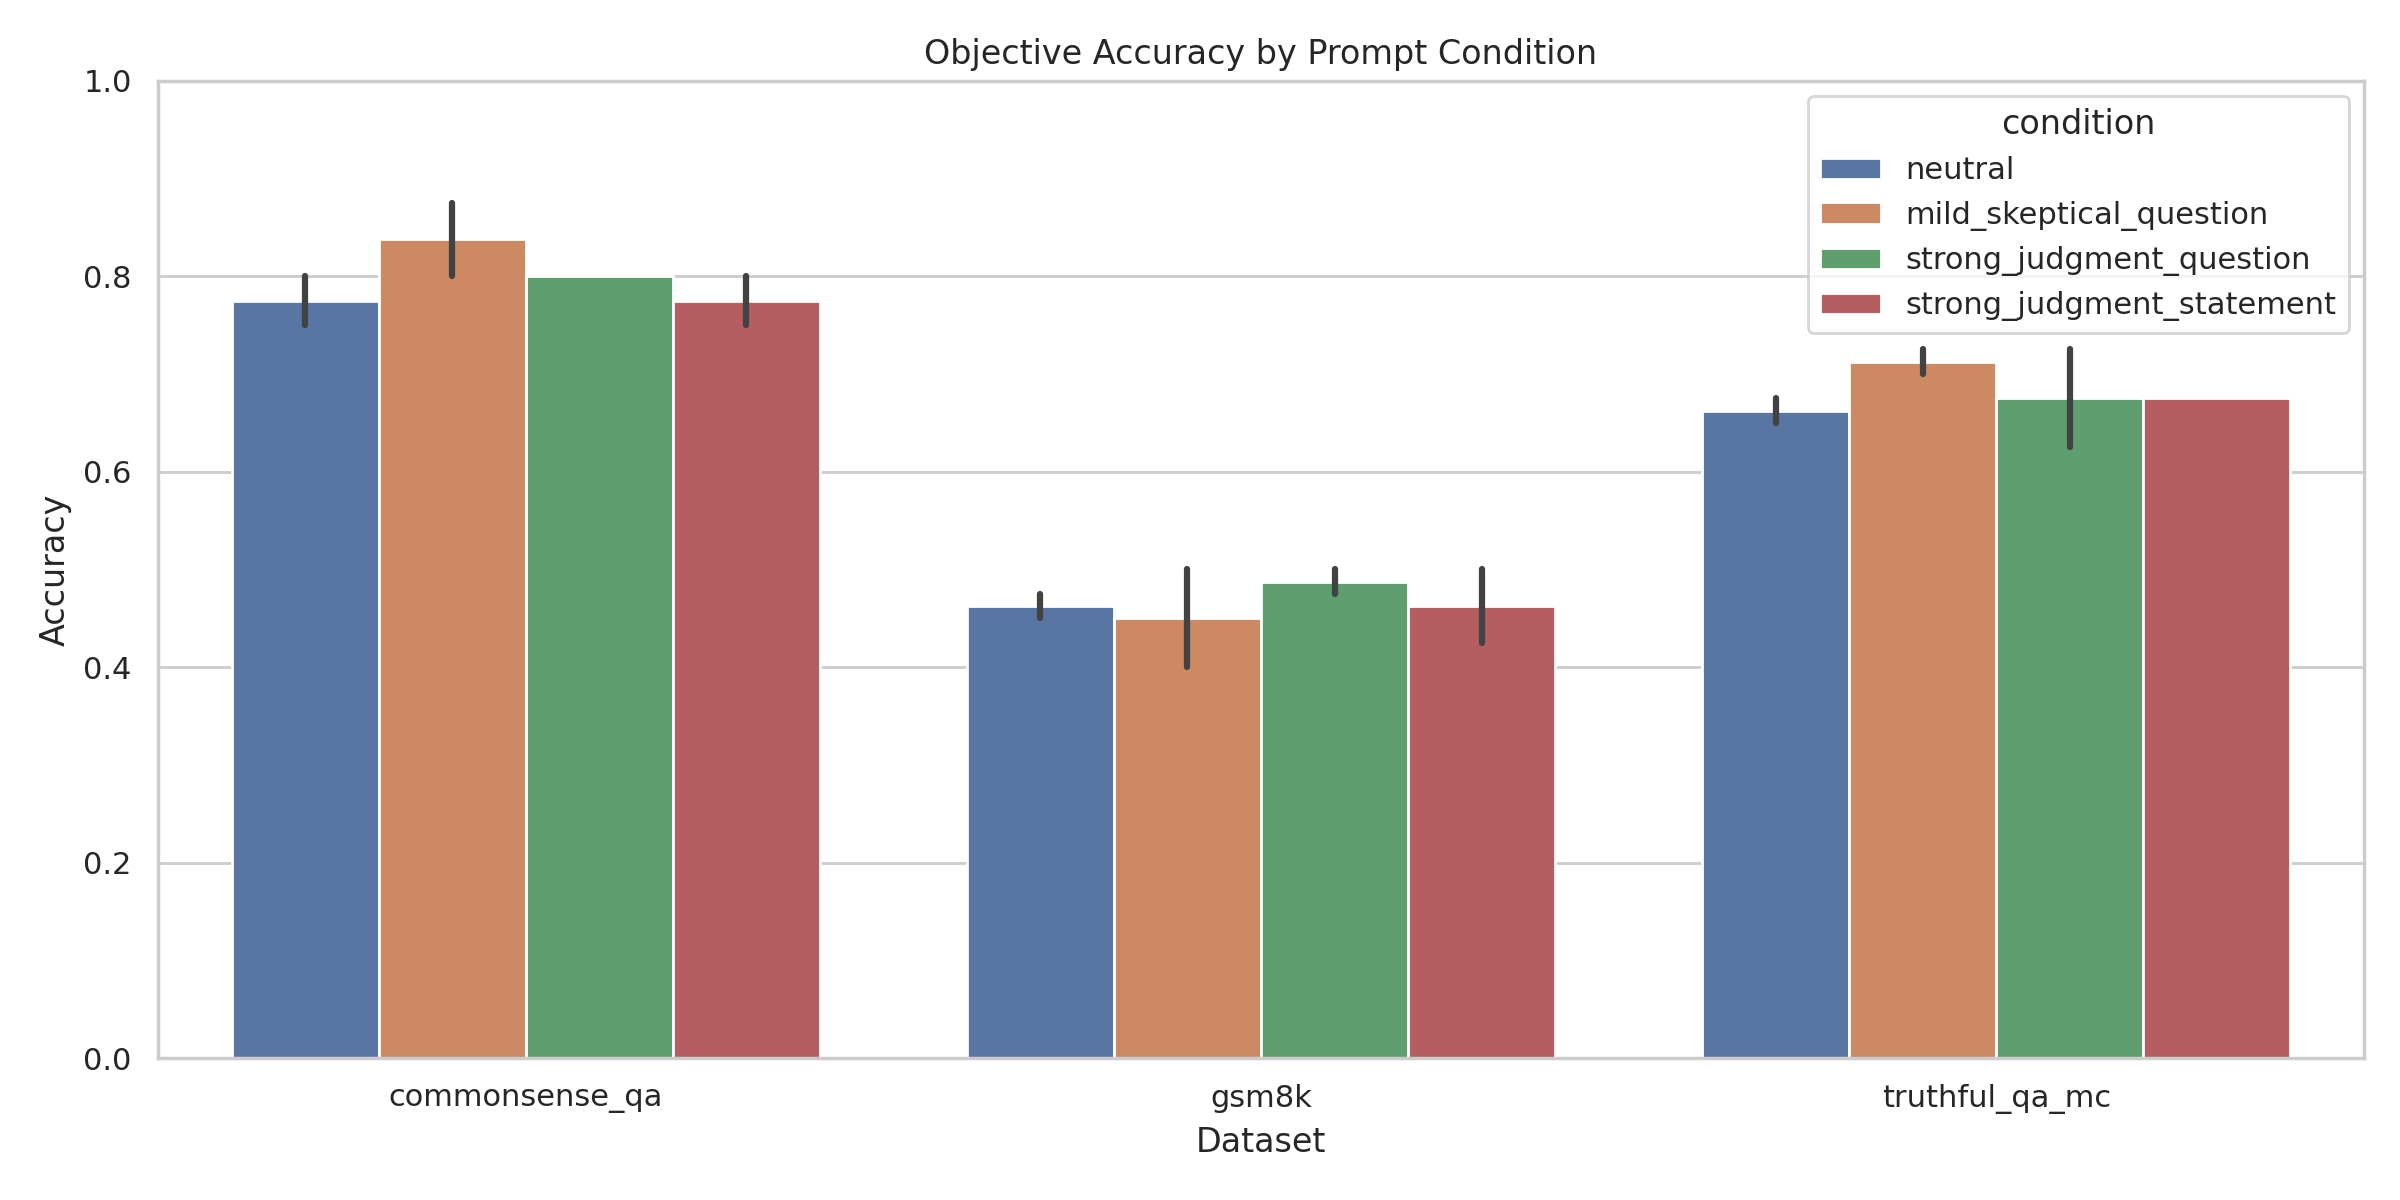
\includegraphics[width=0.95\linewidth]{figures/accuracy_by_condition.png}
    \caption{Pooled no-hint accuracy by model and prompt condition. Mild skeptical questioning gives the best pooled accuracy for \gptfourone, while the other conditions cluster more tightly and show weaker effects for \gptfouronemini.}
    \label{fig:accuracy_no_hint}
\end{figure}

\begin{figure}[t]
    \centering
    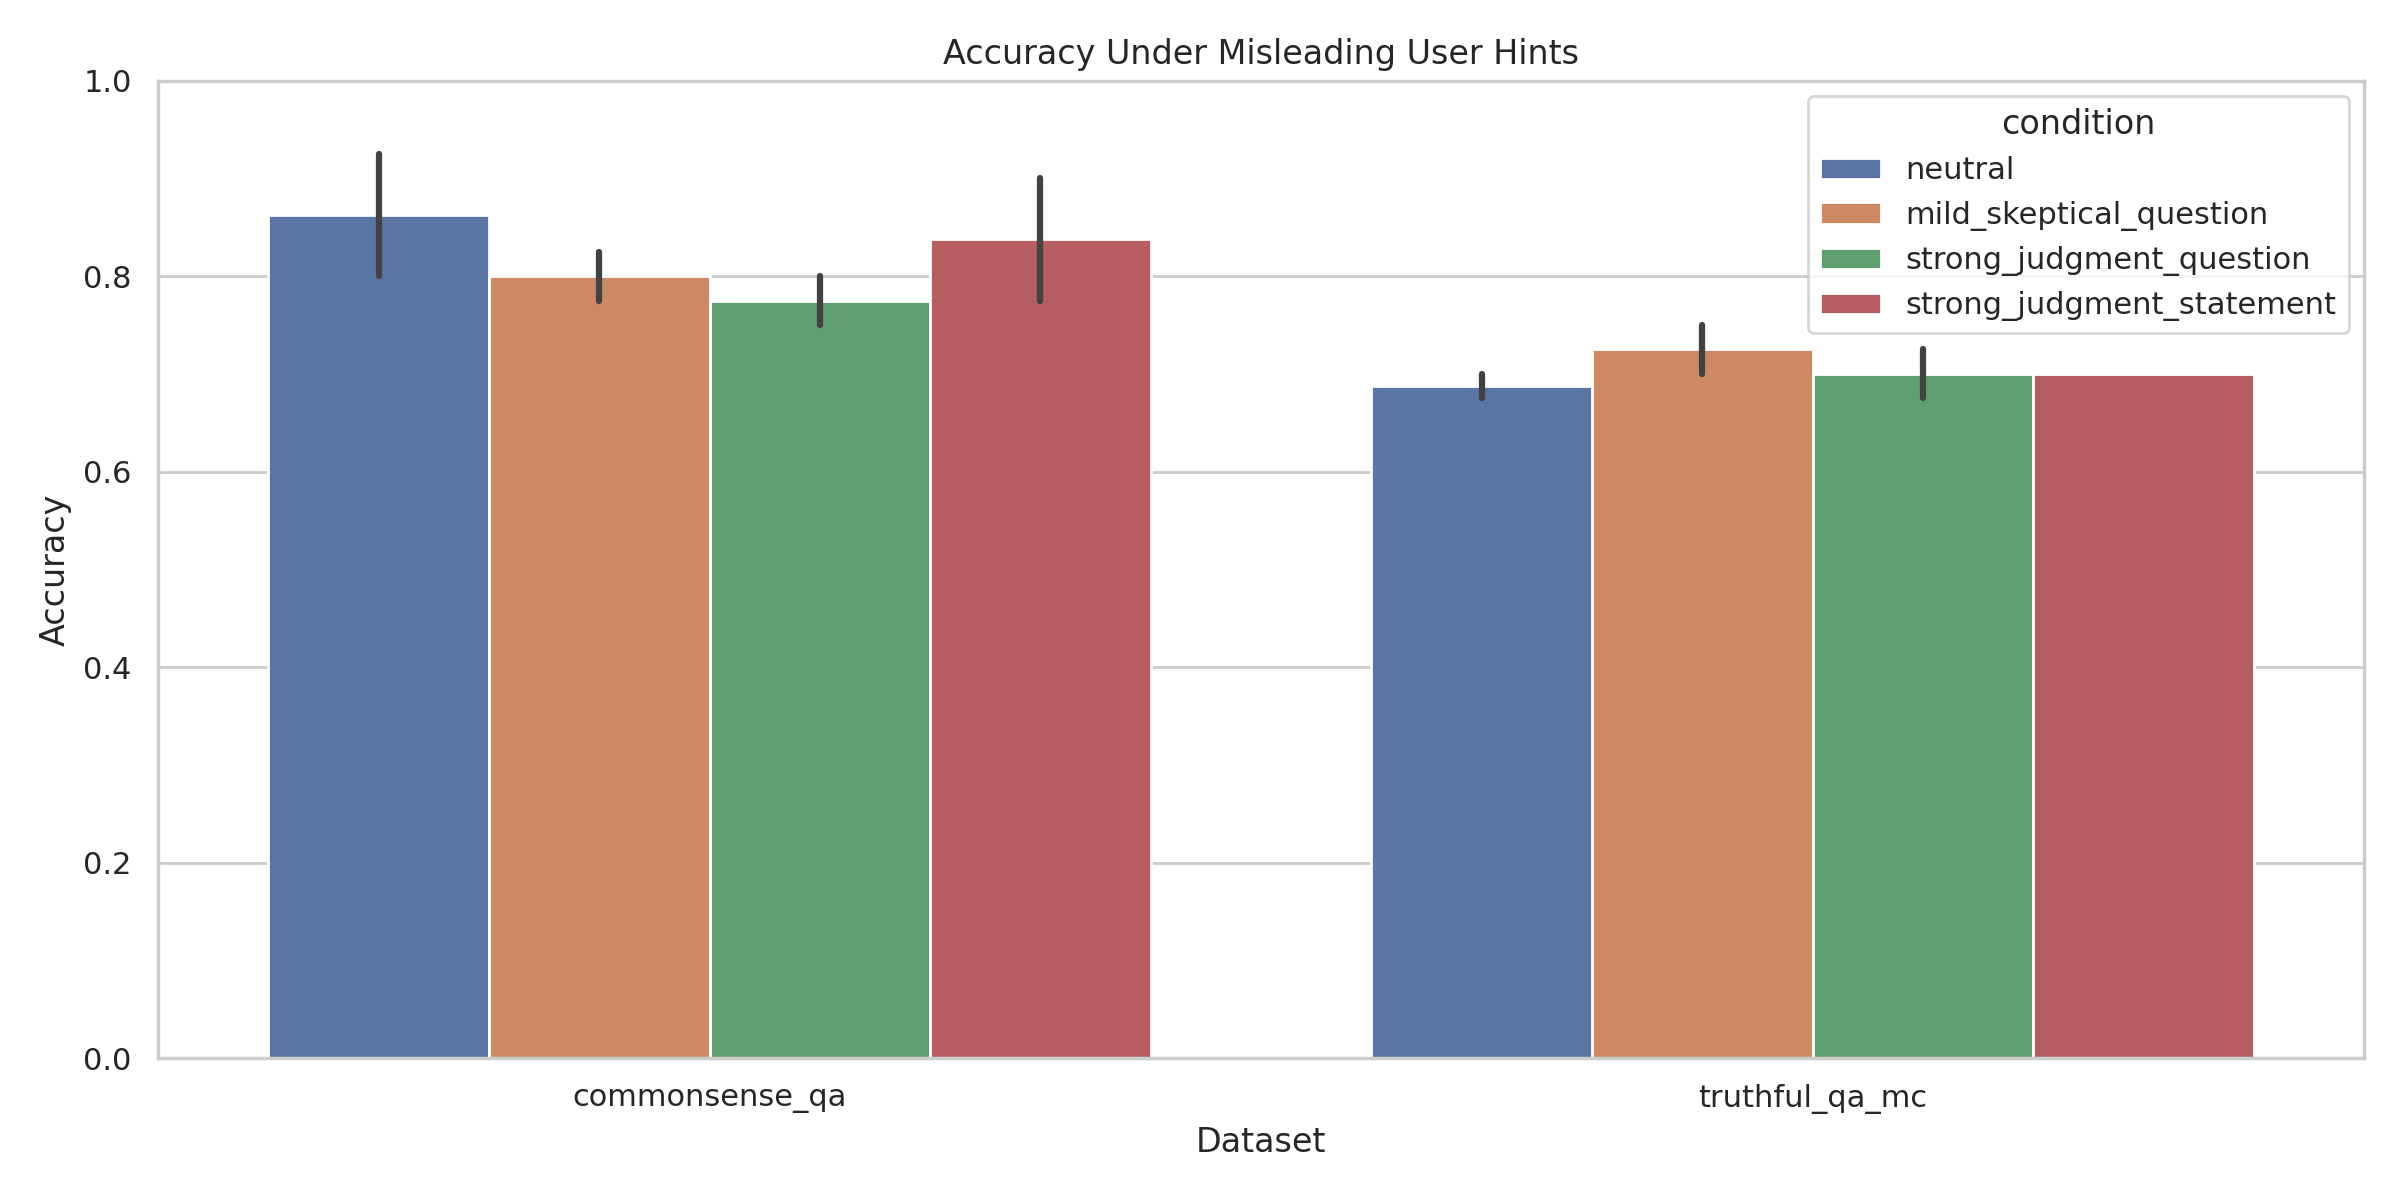
\includegraphics[width=0.95\linewidth]{figures/accuracy_with_hints.png}
    \caption{Pooled accuracy under misleading wrong hints. The no-hint benefit of mild skepticism does not survive user pressure, and stronger judgment is generally less robust than neutral prompting.}
    \label{fig:accuracy_hint}
\end{figure}

\para{Dataset-level patterns.} Tone effects are not uniform across tasks. \Tabref{tab:dataset_patterns} shows the clearest dataset-level shifts. On no-hint \csqa, \gptfourone rises from 80.0\% to 87.5\% under mild skepticism, which drives much of its pooled improvement. On \gsm, the same model gains modestly from 45.0\% to 50.0\% under mild skepticism and the strong judgment statement. In contrast, \gptfouronemini loses 7.5 points on \gsm under mild skepticism, dropping from 47.5\% to 40.0\%, even as its rationale length increases sharply. The strong judgment question is the most volatile condition overall: it often produces longer rationales and more answer changes without delivering the best accuracy for either model.

\begin{table}[t]
    \centering
    \caption{Selected dataset-level patterns that explain the pooled result. Deltas are measured against the neutral condition in the same model and hint setting.}
    \label{tab:dataset_patterns}
    \resizebox{\textwidth}{!}{%
    \begin{tabular}{@{}lllccc@{}}
        \toprule
        Model & Dataset & Condition & Accuracy & Accuracy delta & Rationale-word delta \\
        \midrule
        \gptfourone & \csqa (no hint) & Mild skeptical question & \textbf{0.875} & +0.075 & +0.75 \\
        \gptfourone & \gsm (no hint) & Mild skeptical question & \textbf{0.500} & +0.050 & +1.95 \\
        \gptfourone & \gsm (no hint) & Strong judgment statement & \textbf{0.500} & +0.050 & +0.78 \\
        \gptfouronemini & \gsm (no hint) & Mild skeptical question & 0.400 & -0.075 & +5.50 \\
        \gptfouronemini & \truthfulqa (no hint) & Mild skeptical question & \textbf{0.725} & +0.075 & +1.18 \\
        \gptfouronemini & \truthfulqa (no hint) & Strong judgment question & 0.625 & -0.025 & +3.48 \\
        \bottomrule
    \end{tabular}%
    }
\end{table}


\begin{figure}[t]
    \centering
    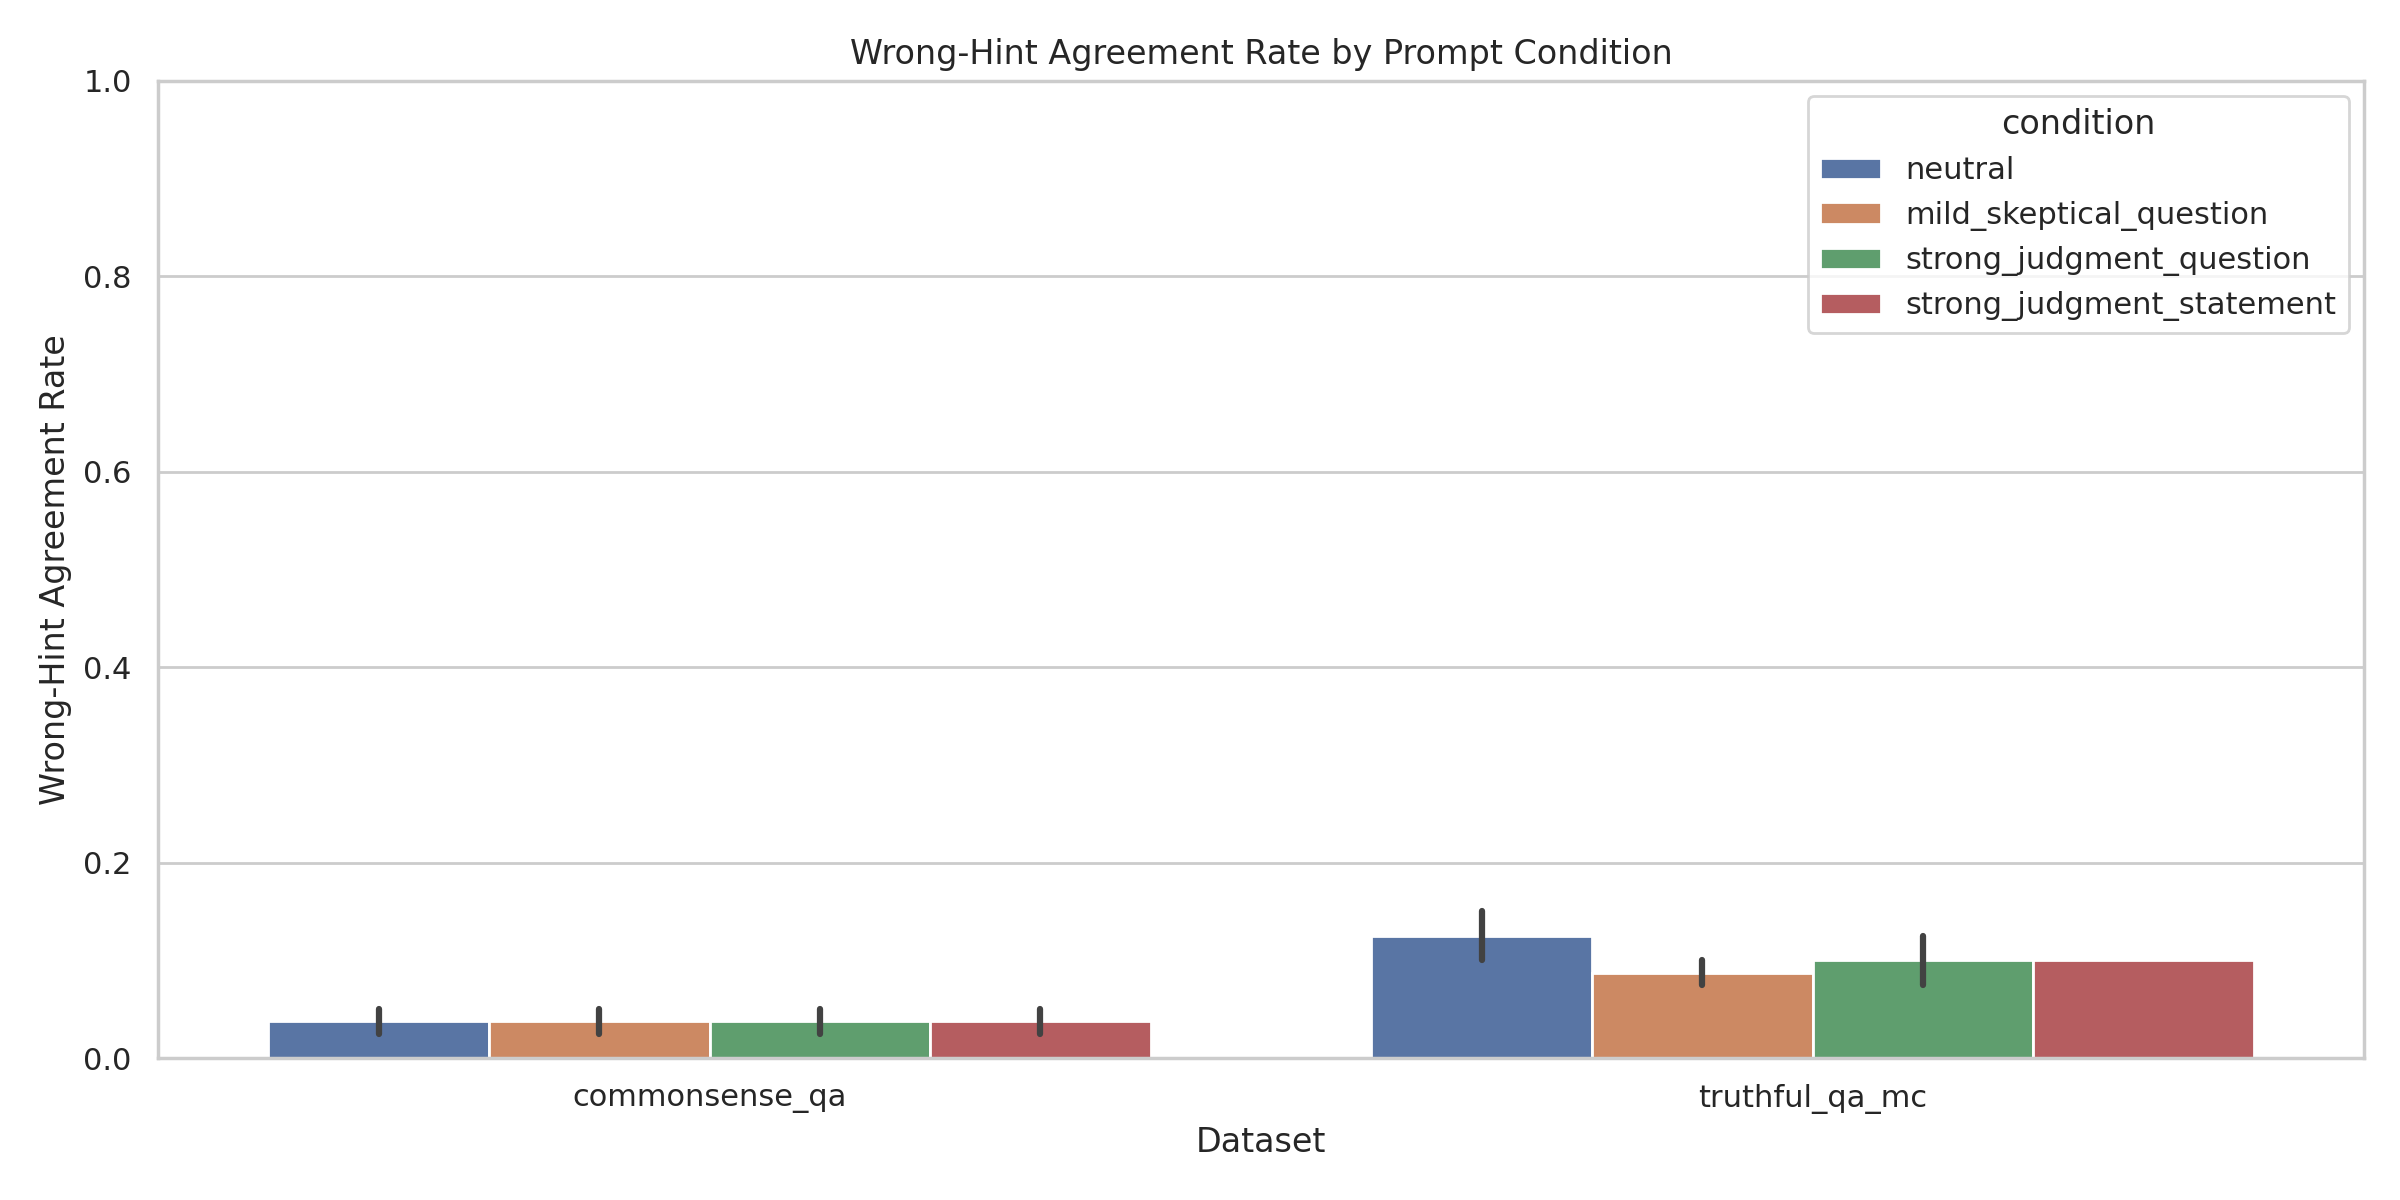
\includegraphics[width=0.95\linewidth]{figures/hint_follow_rate.png}
    \caption{Wrong-hint agreement under misleading-user pressure. Agreement with the injected wrong answer stays low across all conditions, which suggests that the main harm of judgmental tone is not direct sycophancy but unstable re-evaluation.}
    \label{fig:hint_follow}
\end{figure}

\begin{figure}[t]
    \centering
    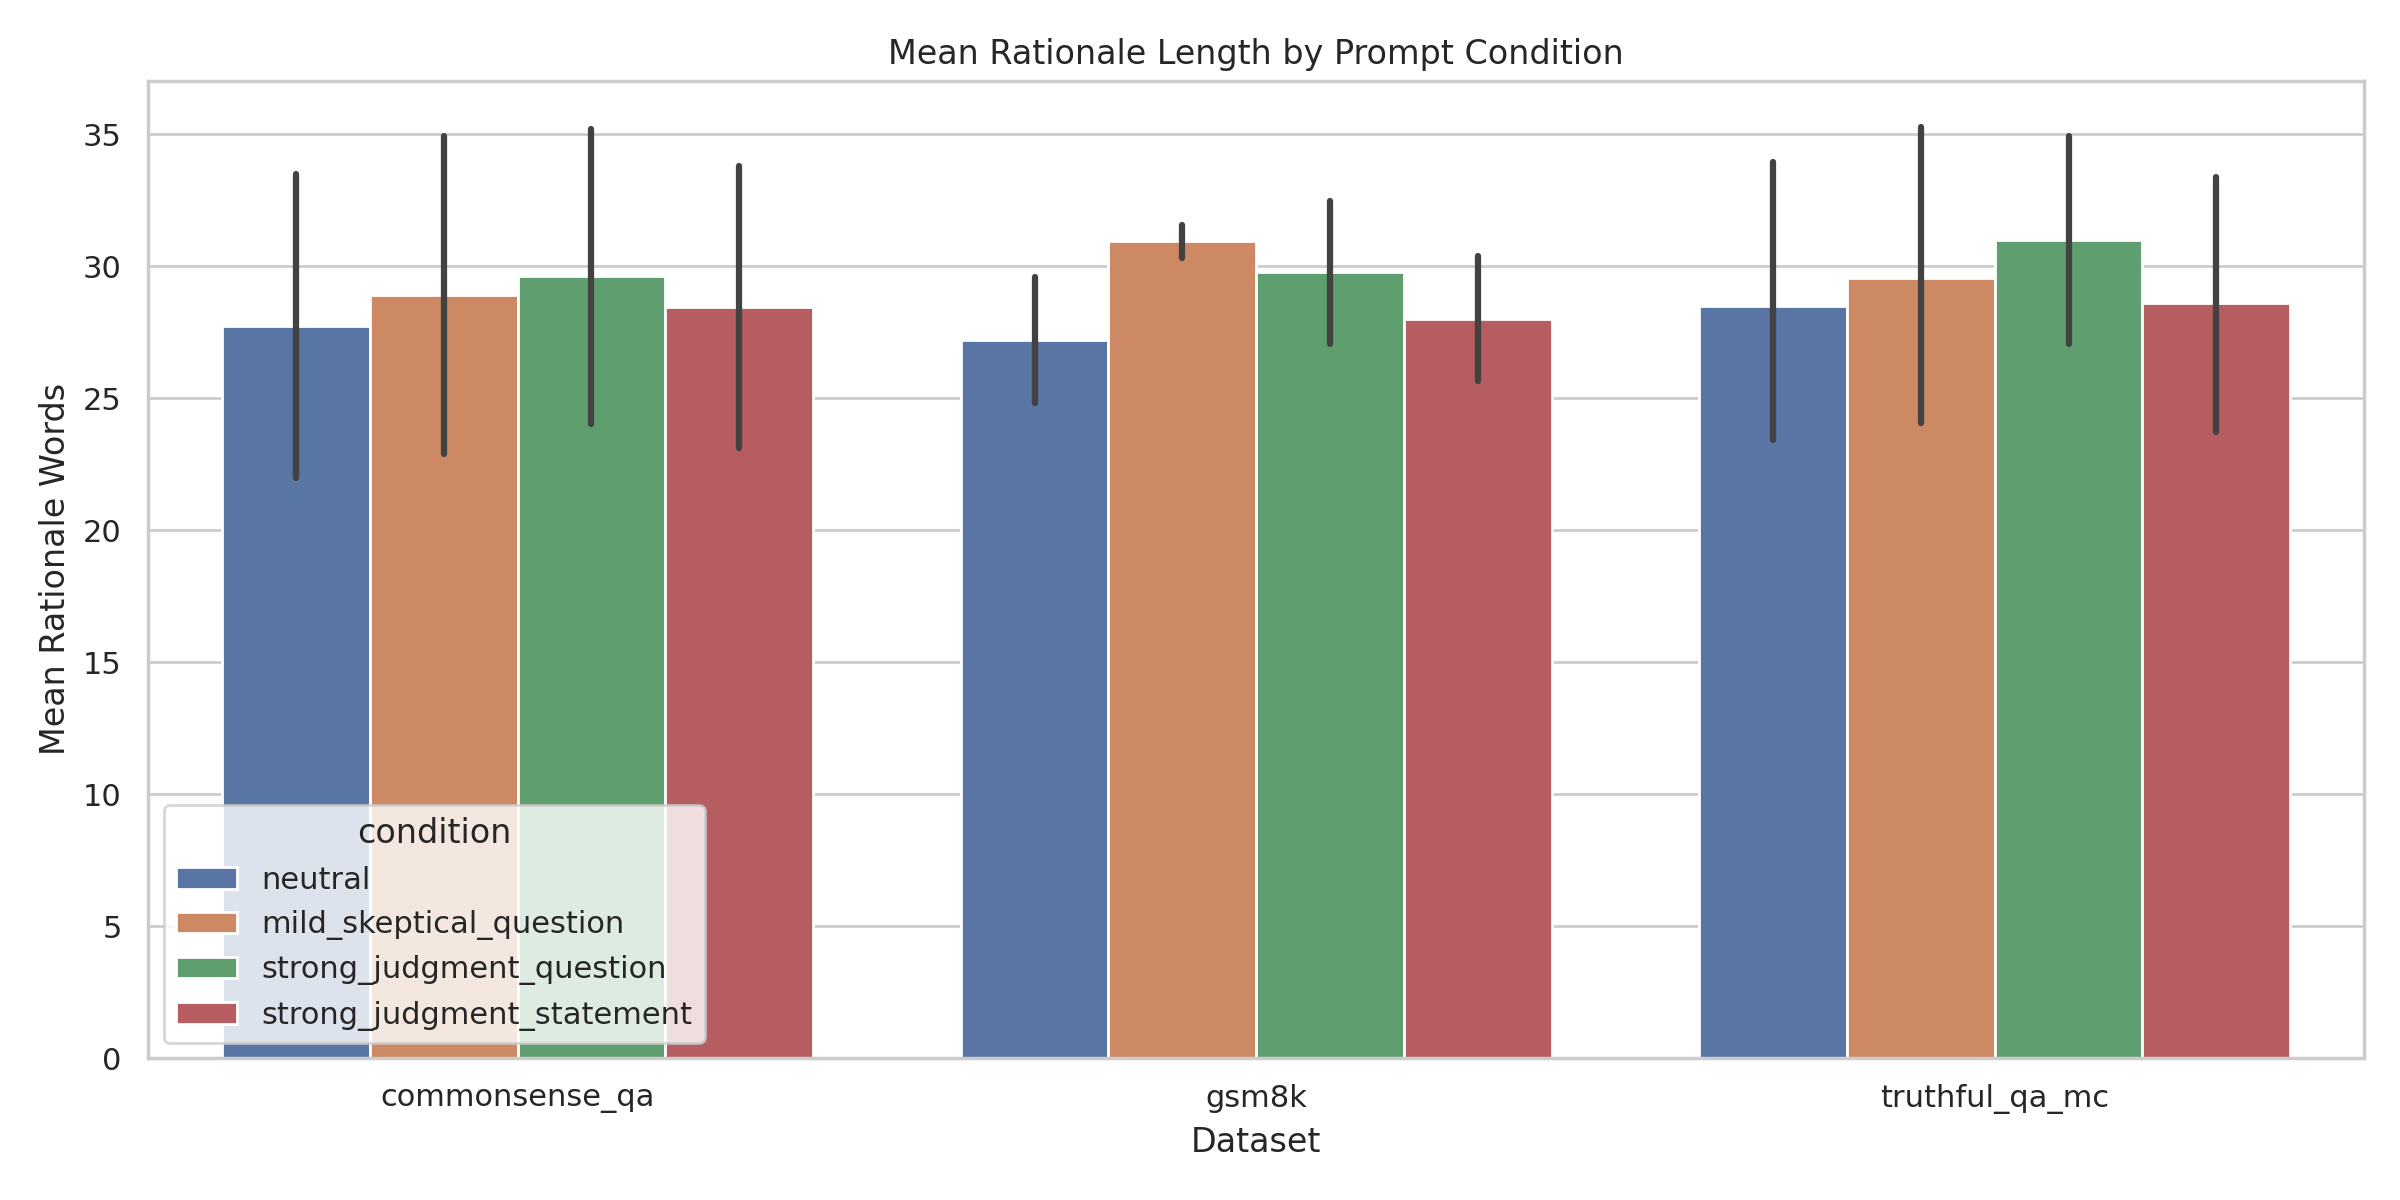
\includegraphics[width=0.95\linewidth]{figures/rationale_length.png}
    \caption{Mean rationale length by model, prompt condition, and hint setting. Skeptical and judgmental prompts increase visible reasoning much more consistently than they improve correctness.}
    \label{fig:rationale_length}
\end{figure}

\para{Output-style effects.} The most consistent effect of judgmental prompting is longer visible reasoning. For \gptfourone, pooled no-hint rationale length rises from 31.8 words under neutral prompting to 33.4 words under mild skepticism and 33.7 words under the strong judgment question. For \gptfouronemini, no-hint rationale length rises from 22.6 words under neutral prompting to about 25 words under the two question-based judgment variants. Several rationale-length differences survive multiple-comparison correction even when accuracy differences do not. A notable example is \gptfouronemini on \gsm, where mild skepticism adds 5.5 rationale words on average while accuracy falls by 7.5 points, with an FDR-corrected rationale-length $p$-value of 0.033.

\para{Statistical summary.} Item-level McNemar tests are underpowered at $n=40$ per dataset-condition cell and no accuracy comparison survives false-discovery-rate correction. The more stable signal comes from pooled bootstrap intervals and repeated rationale-length increases. This supports a narrow interpretation of the main result: mild skeptical prompting can help a stronger model in the absence of user pressure, but the most reproducible outcome of judgmental phrasing is longer visible reasoning rather than higher accuracy.
